\section{Summary}
1. However CouchDB itself has an opinionated implementation of MapReduce - which is used to build B+indexes instead of result sets as in hadoop. As such CouchDB's MapReduce is only useful when querying for analytics of a numerical nature.

2. CouchDB query times go down with more cluster nodes.

3. CouchDB is good for ... xxx


\subsection{Correlation analysis}
The results for \textit{Run 1} and \textit{Run 2} have been summarized in the graphs in Figure \ref{run1-chart1}; several courses were picked at random to show correlation between course grades and student benchmarks. The results show that in general, higher benchmarking scores are indicative of higher course results overall. Some of the benchmarks show stronger correlation to grade results than other, as seen by steeper trendline gradient.



\begin{figure}[H]
    \centering
    \begin{mdframed}
        \centering
        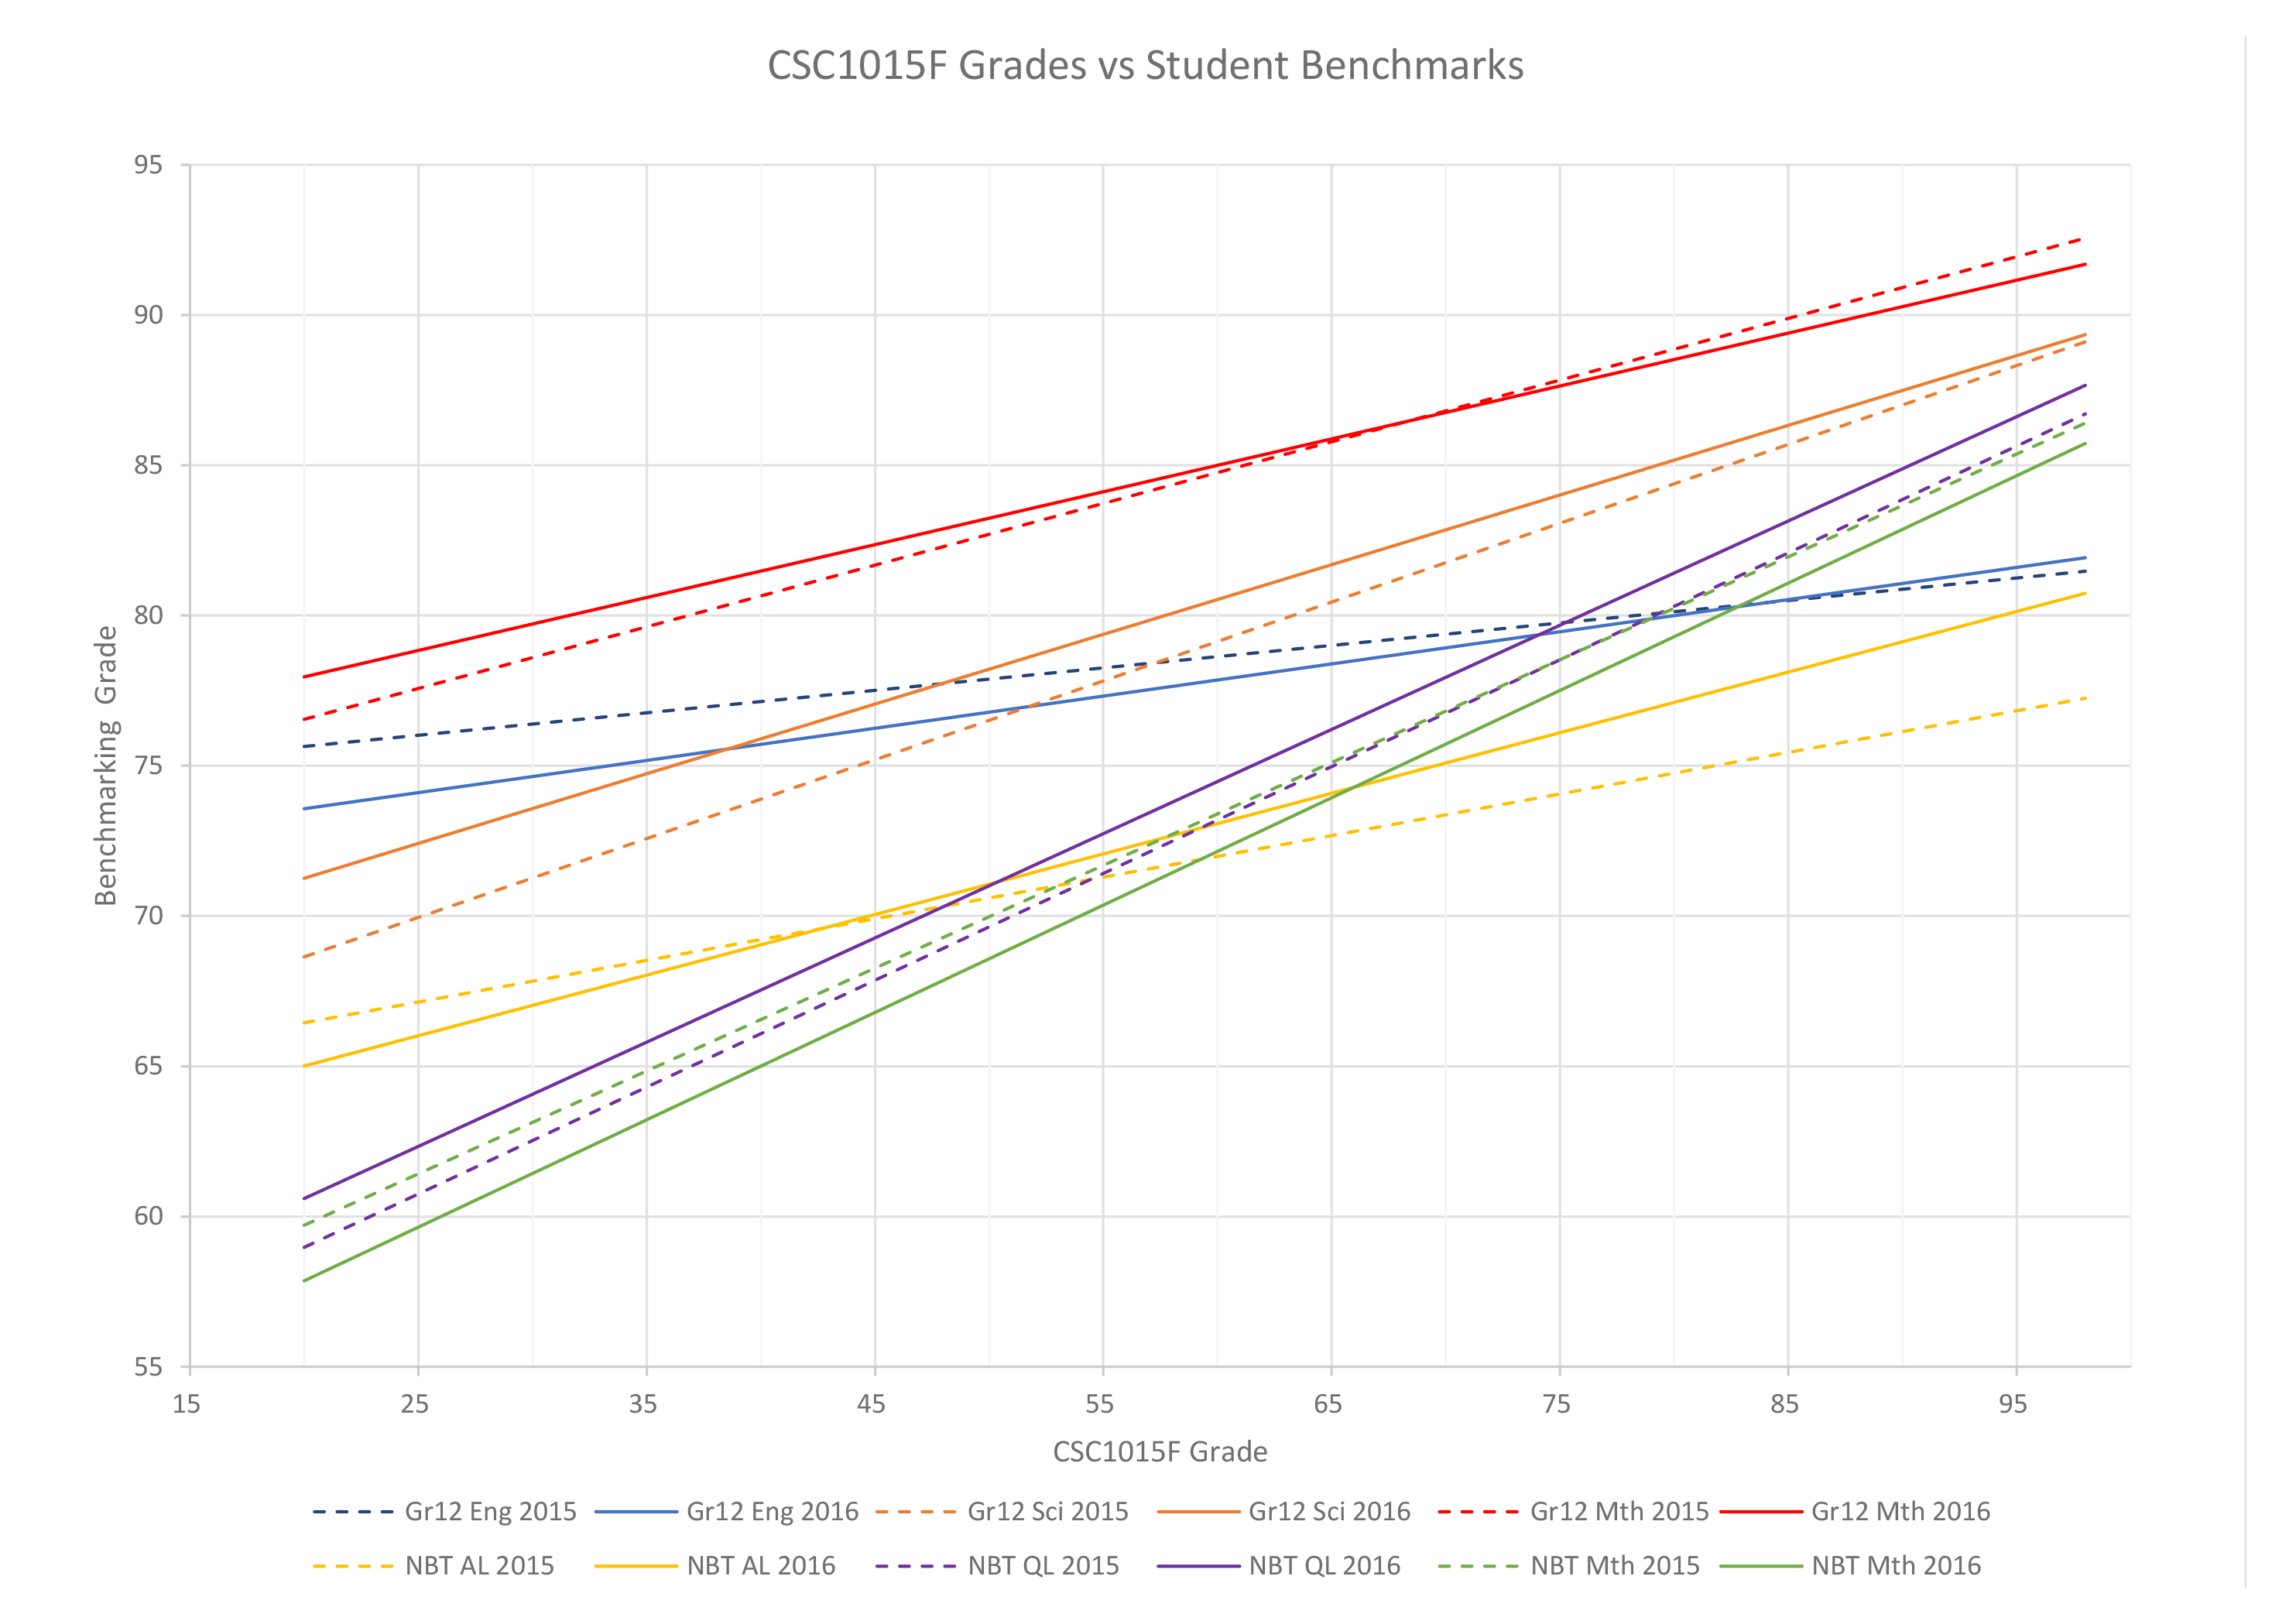
\includegraphics[scale=0.55]{./resources/figures/run1-chart1.png}
    \end{mdframed}
    \caption[CSC1015 grade vs benchmark correlation]{\textbf{Figure \ref{run1-chart1}: Correlation between student benchmarks and CSC1015F results.} This graph shows benchmark scores plotted against the final CSC1015F grade. Datasets focus on a single benchmark, so a trendline shows the correlation between a single benchmark and final grades.}
    \label{run1-chart1}
\end{figure}



\begin{table}[h]
    \begin{threeparttable}
        \textbf{Table \ref{performance-analysis}}\par\medskip\par\medskip
        \caption[Software performance analysis]{Running time analysis of \textit{nETL} tasks and CouchDB MapReduce indexing}
        \label{performance-analysis}
        \begin{tabularx}{\textwidth}{>{\hsize=1\hsize}Y>{\hsize=1\hsize}X>{\hsize=1\hsize}X>{\hsize=1\hsize}X>{\hsize=1\hsize}X}
            \toprule
            \mC{c}{}                                               & \mC{c}{Run 1} & \mC{c}{Run 2} & \mC{c}{Run 3} & \mC{c}{Run 4} \\
            \midrule
            Demographic lines extracted                            & 12 219        & 12 219        & 12 219        &               \\
            Demographic lines loaded                               & 1 381         & 9 874         & 595           &               \\
            Demographic task time (sec)\tnote{\textsuperscript{1}} & 2.488         & 3.114         & 6.755         &               \\
            Grade lines extracted                                  & 513 872       & 513 872       & 513 872       &               \\
            Grade lines loaded                                     & 1 891         & 79 849        & 738           &               \\
            Grade task time (sec)\tnote{\textsuperscript{1}}       & 37.684        & 42.001        & 97.221        &               \\
            Events lines extracted                                 & -             & -             & 44 420 508    &               \\
            Events lines loaded                                    & -             & -             & 661 555       &               \\
            Events task time (sec)\tnote{\textsuperscript{1}}      & -             & -             & 2 225.44      &               \\
            CouchDB footprint (MB)\tnote{\textsuperscript{2}}      & 0.9           & 23.2          & 172.1         &               \\
            View calculation time (sec)\tnote{\textsuperscript{3}} & 0.685         & 49.042        & 340.413       &               \\
            View size (MB)                                         & 0.813         & 143           & 521           &               \\
            \bottomrule
        \end{tabularx}
        \scriptsize
        \begin{tablenotes}
            \item[\textsuperscript{1}]Tasks are run asynchronously, so time taken includes processing of other tasks in this run. Task run times are printed out to the log
            \item[\textsuperscript{2}]This is representative of the amount of data processed by \textit{nETL}
            \item[\textsuperscript{3}]CouchDB views are calculated per shard. By default a database contains 8 shards (even in single node mode). The log file shows start and end times of view calculations for each shard, the time is taken as time the first shard starts indexing, to the time the last shard stops indexing.
        \end{tablenotes}
    \end{threeparttable}
\end{table}

